% CAP description for Combo Box
\begin{itemize}
\item A \bxname{combo box} is a component which consists of a field or button and a drop down list:

\begin{figure}
\begin{center}
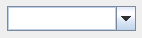
\includegraphics{PS/Combobox}
\caption{Combo Box}
\label{Combobox}
\end{center}
\end{figure}


  \item When the field or button is clicked, the list opens, allowing you to select one of a number of values.
\end{itemize}


Because the comma (,) is a special symbol for combo boxes, if you want to use a comma as part of your parameter value, you have to mask it. See the section later in this document \bxpref{specialchar} for more details. 

\textbf{Mapping combo boxes}

In the \gdomm{}, a combo box to be mapped looks like this:

\begin{figure}
\begin{center}
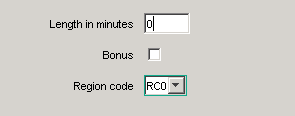
\includegraphics{PS/Mapcombobox}
\caption{Combo Box}
\label{mapcombobox}
\end{center}
\end{figure}

\bxwarn{If you execute a \bxname{click in component} or \bxname{click} action on a combo box, please be aware that the combo box will then be active, and must be deactivated (e.g. by pressing escape) before continuing with other steps (e.g. clicking buttons) in the test.}
